
\usepackage{fancyhdr}
\usepackage{lastpage}
\usepackage[utf8]{inputenc}

% Minted for syntax highliting
\usepackage{minted}
\usemintedstyle{tango}

% 
\usepackage[T1]{fontenc}
\usepackage{lmodern}

\usepackage{calc}
\usepackage{bytefield}

\usepackage{listings}
\usepackage{amsmath}

\usepackage{tikz}
\usetikzlibrary{automata,arrows,topaths,calc,positioning}
 
\usepackage{syntax}
\grammarindent=2cm


% Headers/footers styling
\pagestyle{fancy}
\fancyhf{}
\renewcommand{\headrulewidth}{0pt}

% Footer
\lfoot{ID1019}
\cfoot{KTH}
\rfoot{\thepage \hspace{1pt} / \pageref{LastPage}}

%\newcommand{\defaultpagestyle}{\thispagestyle{plain}}
\newcommand{\defaultpagestyle}{\thispagestyle{fancy}}



\usetikzlibrary{shapes.misc}


\title[ID1019 MIPS]{MIPS}

\author{Johan Montelius}
\institute{KTH}
\date{\semester}

\begin{document}

\begin{frame}
\titlepage
\end{frame}

\begin{frame}{The MIPS architecture}
 
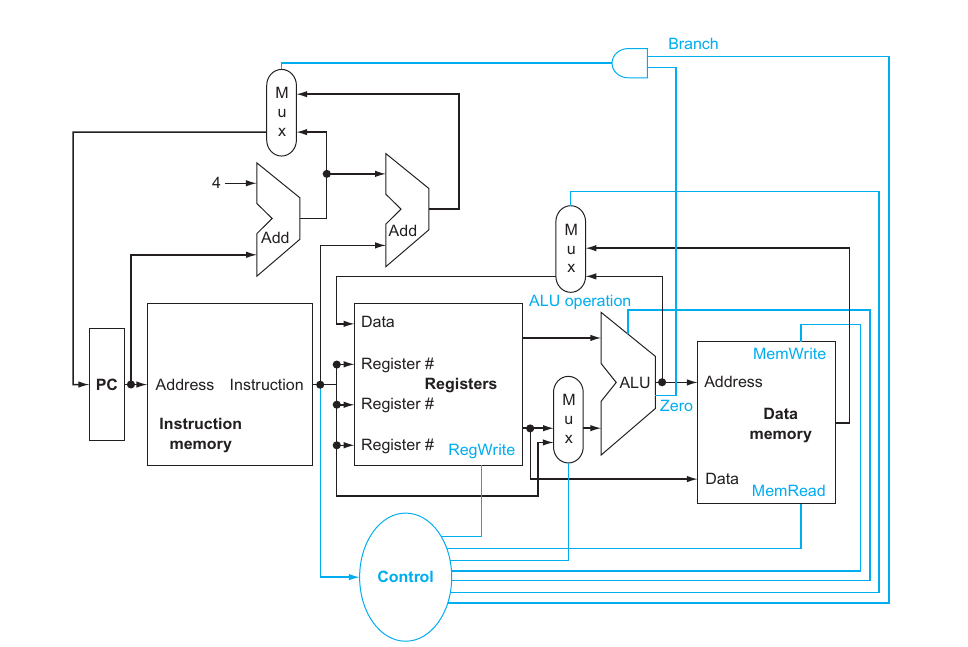
\includegraphics[scale=0.4]{mips.png}  

{\em From ``Computer Organization and Design'', Patterson and Hennessy, Fig 4.2}
\end{frame}

\begin{frame}{The data flow}

\begin{figure}
  \centering 
  \begin{tikzpicture}[unit/.style={rectangle, very thick, minimum height=1cm, minimum width=2cm, text centered}]

%Nodes
\node[unit]    (instr)                      {Instruction};
\node[unit]    (reg)       [right=of instr] {Register};
\node[unit]    (alu)       [right=of reg]   {ALU};
\node[unit]    (mem)       [right=of alu]   {Memory};
\node[unit]    (brn)       [above=of alu]   {Branch};
\node[unit]    (ctrl)       [below=of reg]   {Controller};
%Lines 
\draw[->, dash dot] (instr.east) -- (reg.west);
\draw[->, dashed] (instr.south) .. controls +(down:1cm) and +(left:1cm) ..  (ctrl.west);

\draw[->] (reg.east) -- (alu.west);

\draw[->] (alu.east) -- (mem.west);
\draw[->, dashed] (alu.north) -- (brn.south);

\draw[->] (instr.north) .. controls +(up:1cm) and +(left:1cm) .. (brn.west);
\draw[->] (instr.south) .. controls +(down:1cm) and +(down:1cm) .. (alu.south);

\draw[->] (reg.south) .. controls +(down:1cm) and +(down:1cm) .. (mem.south);

\draw[->, dash dot] (brn.north) .. controls +(up:2cm) and +(left:3cm) .. (instr.west);
\draw[->] (mem.north) .. controls +(up:1cm) and +(up:1cm) .. (reg.north);

  \end{tikzpicture}
  \caption{The data flow of the processor.} \label{fig:flow}
\end{figure}

\end{frame}

\begin{frame}{sequence diagram}
  
\begin{figure}
  \centering 
  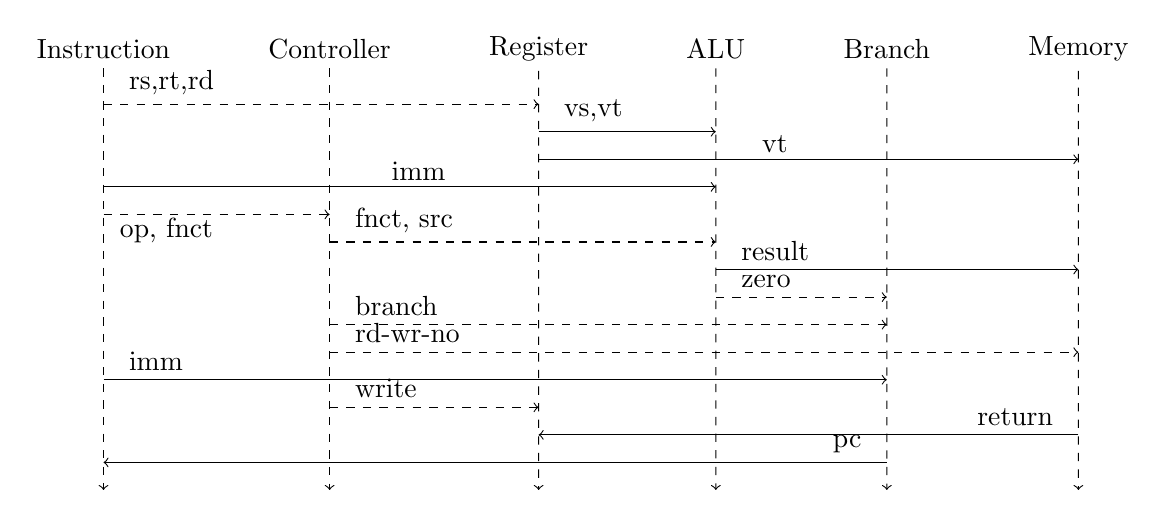
\begin{tikzpicture}[scale=0.7, frw/.style={xshift=0.2cm, yshift=-0.1, anchor= south west}, bkw/.style={xshift=-0.2cm, anchor= south east}]

    \node[]                 (instr) {Instruction};
    \node[right = of instr] (ctrl)  {Controller};
    \node[right = of ctrl]  (reg)   {Register};
    \node[right = of reg]   (alu)   {ALU};    
    \node[right = of alu]   (brn)   {Branch};
    \node[right = of brn]   (mem)   {Memory};    
    
    
    \draw[->, dashed] (instr) -- ($ (instr) - (0,8)$);
    \draw[->, dashed] (reg) -- ($ (reg) - (0,8)$);
    \draw[->, dashed] (ctrl) -- ($ (ctrl) - (0,8)$);
    \draw[->, dashed] (alu) -- ($ (alu) - (0,8)$);
    \draw[->, dashed] (brn) -- ($ (brn) - (0,8)$);    
    \draw[->, dashed] (mem) -- ($ (mem) - (0,8)$);    
    
    \draw[->, dashed] ($(instr) - (0,1)$) node[frw]{rs,rt,rd} --  ($(reg)  - (0,1)$);

    \draw[->] ($(reg) - (0,1.5)$) node[frw]{vs,vt} --  ($(alu)  - (0,1.5)$);

    \draw[->] ($(reg) - (0,2.0)$) node[xshift=3cm, yshift=0.2cm]{vt} --  ($(mem)  - (0,2.0)$);
    

    \draw[->] ($(instr) - (0,2.5)$) node[xshift=4cm, yshift=0.2cm]{imm} --  ($(alu)  - (0,2.5)$);

    \draw[->, dashed] ($(instr) - (0,3.0)$) node[xshift=0.8cm, yshift=-0.2cm]{op, fnct}  --   ($(ctrl)  - (0,3.0)$);

    \draw[->, dashed] ($(ctrl) - (0,3.5)$) node[frw]{fnct, src} --  ($(alu)  - (0,3.5)$);    

    \draw[->] ($(alu) - (0,4.0)$) node[frw]{result} --  ($(mem)  - (0,4.0)$);

    \draw[->, dashed] ($(alu) - (0,4.5)$) node[frw]{zero} --  ($(brn)  - (0,4.5)$);    

    \draw[->, dashed] ($(ctrl) - (0,5.0)$) node[frw]{branch} --  ($(brn)  - (0,5.0)$);

    \draw[->, dashed] ($(ctrl) - (0,5.5)$) node[frw]{rd-wr-no} -- ($(mem)  - (0,5.5)$);    

    \draw[->] ($(instr) - (0,6.0)$) node[frw]{imm} --  ($(brn)  - (0,6.0)$);    
    
    \draw[->, dashed] ($(ctrl) - (0,6.5)$) node[frw]{write}  -- ($(reg)  - (0,6.5)$);    

    \draw[->] ($(mem) - (0,7.0)$) node[bkw]{return}  -- ($(reg)  - (0,7.0)$);

    \draw[->] ($(brn) - (0,7.5)$) node[bkw]{pc}  -- ($(instr)  - (0,7.5)$);            
    
  \end{tikzpicture}
\end{figure}

\end{frame}

\begin{frame}{instruction format}

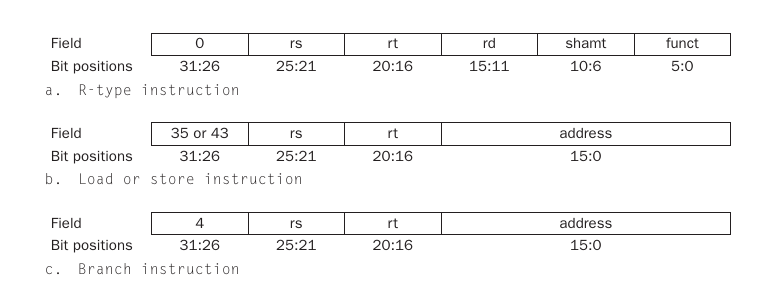
\includegraphics[scale=0.6]{rtype.png}  

\vspace{20pt}
{\em From ``Computer Organization and Design'', Patterson and Hennessy, Fig 4.14}
\end{frame}

\begin{frame}[fragile]{instruction encoding}

 \begin{verbatim}
   {:add, rd, rs, rt} -> 
      <<@aop::6, rs::5, rt::5, rd::5, 0::5, @add::6>>
 \end{verbatim}

\end{frame}

\begin{frame}[fragile]{instruction decoding}

 \begin{lstlisting}
	<<op::6, rs::5, rt::5, rest::binary>>  = instr
	<<rd::5, _shamt::5, fnct::6>> = rest
	<<imm::integer-signed-16>>  = rest
  \end{lstlisting}
\end{frame}

\begin{frame}{Pipelined architecture}
 
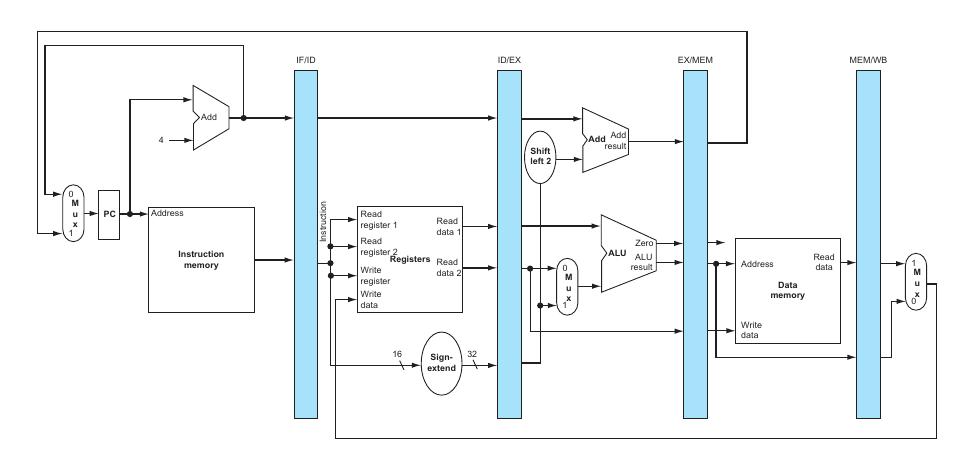
\includegraphics[scale=0.5]{pipeline.png}  

\vspace{20pt}
{\em From ``Computer Organization and Design'', Patterson and Hennessy, Fig 4.35}
\end{frame}


\end{document}



